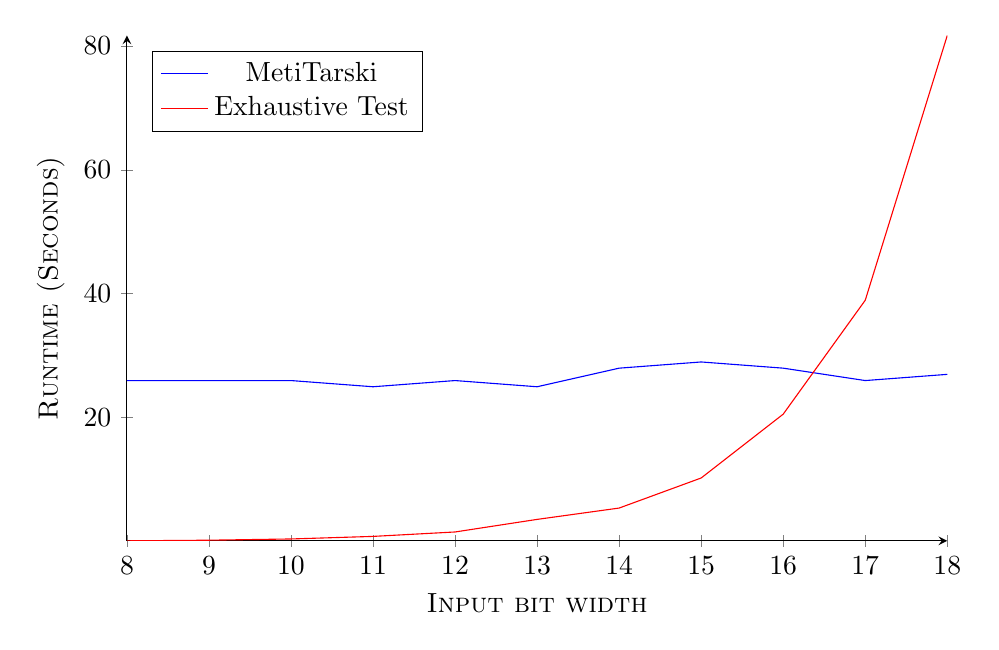
\begin{tikzpicture}
\begin{axis}[
    axis lines = left,
    xlabel = \textsc{Input bit width},
    ylabel = \textsc{Runtime (Seconds)},
    legend pos=north west,height=80mm, width=120mm]

\addplot[
    color=blue,
    ]
    coordinates {(8 ,26)(9 ,26)(10,26)(11,25)(12,26)(13,25)(14,28)(15,29)(16,28)(17,26)(18,27)   };
    \addlegendentry{MetiTarski}
\addplot[color=red,
        ]
        coordinates{(8 ,0.14548254013061523 )
(9 ,0.24578046798706055 )(10,0.4463155269622803  )
(11,0.8605005741119385  )(12,1.574721336364746   )
(13,3.603602409362793   )(14,5.432856559753418)
(15,10.283031702041626)(16,20.580944299697876)
(17,38.95604610443115)(18,81.67475938796997)

 };
        \addlegendentry{Exhaustive Test}
\end{axis}
\end{tikzpicture}
